\chapter{الاستقلاب الجرثومي والأغشية الحيوية}\label{ch:b2:microbial-metabolism}

املأ أسطوانة زجاجية بوحل بركة، وقليل من الورق الممزق، وصفار بيضة،
وماء، ثم اتركها على حافة نافذة. ففي غضون أسابيع تتطبق في نطق ملونة:
طحالب خضراء في الأعلى، وطبقة صدئة، ونطاق أرجواني، وآخر أخضر أدنى
منه، ووحل أسود من الكبريتيد في القاع. ولم يُضف شيء سوى الضوء. وكل
نطاق جمهرة تعيش على كيمياء مختلفة --- على الأكسجين، أو النترات، أو
الكبريتات، أو الكبريتيد، أو الهدروجين --- ويغذي كل منها الذي يليه.
فالأسطوانة هي العالم الجرثومي مصغرًا: خلايا تكسب طاقتها من أي زوج
من المواد يستطيع تبادل الإلكترونات تقريبًا، وتدير مجتمعةً الدورات
الكيميائية للكوكب. يعرض هذا الفصل منطق تلك الطاقية، وحركية النمو
الجرثومي، والحياة الجماعية للجراثيم على السطوح، وهي الطريقة التي
يعيش بها معظمها فعلًا.

\section{طرائق كسب العيش}

\begin{definition}[أنماط التغذي]\label{def:b2:microbial-metabolism:trophic}
\index{متغذٍّ كيميائي}\index{متغذٍّ ضوئي}\index{متغذٍّ معدني}\index{متغذٍّ عضوي}
يُصنَّف الكائن بثلاثة أجوبة. \emph{مصدر طاقته}: الضوء
(\emph{متغذٍّ ضوئي}) أو التفاعلات الكيميائية (\emph{متغذٍّ كيميائي}).
و\emph{مصدر إلكتروناته}: مواد لاعضوية --- $\mathrm{H_2}$،
$\mathrm{H_2S}$، $\mathrm{NH_4^+}$، $\mathrm{Fe^{2+}}$، الماء ---
(\emph{متغذٍّ معدني}) أو جزيئات عضوية (\emph{متغذٍّ عضوي}).
و\emph{مصدر كربونه}: $\mathrm{CO_2}$ (\emph{ذاتي التغذي}) أو كربون
عضوي (\emph{غير ذاتي التغذي}). فالنباتات والزراقم ذاتية التغذي
ضوئيًا معدنيًا؛ والحيوانات والفطريات و\emph{E.~coli} غير ذاتية
التغذي كيميائيًا عضويًا؛ أما بكتيريا النترتة وأكسدة الكبريت فذاتية
التغذي كيميائيًا معدنيًا، تصنع مادتها العضوية من $\mathrm{CO_2}$
بطاقة تستمدها من أكسدة المعادن، في الظلام. وكل تركيب من هذه تقريبًا
موجود في مكان ما بين بدائيات النوى؛ أما حقيقيات النوى فلا تشغل إلا
اثنين.
\end{definition}

\begin{theorem}[طاقة زوج الأكسدة والإرجاع]\label{thm:b2:microbial-metabolism:redox}
\index{كمون الأكسدة والإرجاع}\index{برج الإلكترونات}
كل استقلاب مولّد للطاقة ينقل إلكترونات من زوج \emph{واهب} إلى زوج
\emph{متقبل}. ولكل زوج كمون معياري $E^{\circ\prime}$ (عند pH 7):
فكلما كان أشد سلبية كان أسهل إعطاءً للإلكترونات. ونقل $n$ مولًا من
الإلكترونات من واهب عند $E_d$ إلى متقبل عند $E_a$ يحرر طاقة حرة
معيارية
\[
\Delta G^{\circ\prime} = -\,n F\,(E_a - E_d), \qquad F = \qty{96.5}{kJ/V/mol},
\]
أي إن المردود يتناسب مع المسافة العمودية بين الزوجين على
\emph{\omterm{thm:b2:microbial-metabolism:redox}{برج الإلكترونات}}. فمع $\mathrm{O_2/H_2O}$ عند \qty{+0.82}{V}
و$\mathrm{CO_2}$/الغلوكوز عند
\qty{-0.43}{V}، تعطي إلكترونات جزيء الغلوكوز الأربعة والعشرون
$24\times 96.5\times 1.25 = \qty{2900}{kJ/mol}$؛ وإذا سُلّمت بدل ذلك
إلى الكبريتات ($\mathrm{SO_4^{2-}/H_2S}$، \qty{-0.22}{V}) لم تعط
الإلكترونات نفسها إلا $24\times 96.5\times 0.21 = \qty{490}{kJ/mol}$.
\end{theorem}
\begin{proof}
من أجل التفاعل: الواهب$_{\text{مرجع}}$ + المتقبل$_{\text{مؤكسد}}$
$\to$ الواهب$_{\text{مؤكسد}}$ + المتقبل$_{\text{مرجع}}$، يكون تغير
الطاقة الحرة هو الشغل الذي يبذله $n$ مولًا من شحنة الإلكترون $nF$
وهي تسقط عبر فرق الكمون $E_a - E_d$، مع اصطلاح الإشارة أن النقل
التلقائي (الإلكترونات نحو الزوج الأكثر إيجابية) له $\Delta G < 0$.
وهذه علاقة نرنست التي درسها مجلد السنة الأولى، مطبقة على نصفي
تفاعل.
\end{proof}

\begin{omfigure}
\begin{tikzpicture}[every node/.style={font=\scriptsize}, y=6cm]
  \draw[thick, ->] (0,-0.55) -- (0,0.95) node[above] {$E^{\circ\prime}$ (V)};
  \foreach \v in {-0.4,-0.2,0,0.2,0.4,0.6,0.8} \draw (-0.08,\v) -- (0.08,\v) node[right, xshift=0.05cm] {\v};
  % donors on the right: value/label position/text
  \foreach \v/\y/\l in {-0.43/-0.49/{$\mathrm{CO_2}$/غلوكوز}, -0.42/-0.40/{$2\mathrm{H^+/H_2}$}, -0.32/-0.31/{$\mathrm{NAD^+/NADH}$}, -0.27/-0.22/{$\mathrm{S^0/H_2S}$}, 0.03/0.03/{فومارات/سكسينات}, 0.34/0.34/{$\mathrm{NO_2^-/NH_4^+}$}}
    { \draw[omDef, thick] (0.8,\v) -- (1.6,\v); \draw[omDef] (1.6,\v) -- (1.85,\y); \node[omDef, anchor=west] at (1.9,\y) {\l}; }
  % acceptors on the left
  \foreach \v/\y/\l in {-0.24/-0.29/{$\mathrm{CO_2/CH_4}$}, -0.22/-0.17/{$\mathrm{SO_4^{2-}/H_2S}$}, 0.43/0.43/{$\mathrm{NO_3^-/NO_2^-}$}, 0.74/0.69/{$\mathrm{NO_3^-/N_2}$}, 0.77/0.77/{$\mathrm{Fe^{3+}/Fe^{2+}}$}, 0.82/0.86/{$\mathrm{O_2/H_2O}$}}
    { \draw[omThm, thick] (-1.6,\v) -- (-0.8,\v); \draw[omThm] (-1.6,\v) -- (-1.85,\y); \node[omThm, anchor=east] at (-1.9,\y) {\l}; }
  \node[omThm, anchor=south] at (-2.4,0.93) {المتقبلات};
  \node[omDef, anchor=south] at (2.4,0.93) {الواهبات};
  % arrows showing two metabolisms
  \draw[->, very thick, omExo!80!black] (4.9,-0.43) -- (4.9,0.80);
  \node[anchor=west, align=left] at (5.0,0.2) {تنفس هوائي\\للغلوكوز: \qty{1.25}{V}،\\\qty{2900}{kJ/mol}};
  \draw[->, very thick, omProp] (4.2,-0.43) -- (4.2,-0.24);
  \node[anchor=north, align=center] at (4.2,-0.52) {إرجاع الكبريتات:\\\qty{0.21}{V}، \qty{490}{kJ/mol}};
  \draw[dashed, gray] (3.5,-0.43) -- (4.9,-0.43);
  \draw[dashed, gray] (3.5,0.82) -- (4.9,0.82);
  \draw[dashed, gray] (3.5,-0.22) -- (4.2,-0.22);
\end{tikzpicture}

{\small \omterm{thm:b2:microbial-metabolism:redox}{برج الإلكترونات}. الواهبات (بالأزرق) مرتبة عند كموناتها
المعيارية؛ والمتقبلات (بالأحمر) كذلك. والاستقلاب سقوط من واهب إلى
متقبل فوقه، ومردوده الطاقي يتناسب مع ارتفاع السقطة: فمن الغلوكوز
إلى الأكسجين سقطة طويلة، ومن الغلوكوز إلى الكبريتات سقطة قصيرة.}
\end{omfigure}

\begin{proposition}[التغذي الكيميائي المعدني]\label{prop:b2:microbial-metabolism:lithotrophy}
\index{تغذٍّ كيميائي معدني}\index{نترتة}
بعض البكتيريا تستمد كل طاقتها من أكسدات لاعضوية، مستعملة الأكسجين
(أو النترات) متقبلًا، وتثبّت $\mathrm{CO_2}$ بما تكسبه من ATP وقدرة
إرجاعية. \emph{مُنَترِتات}: مؤكسدات الأمونيوم
(\emph{Nitrosomonas}) تحول $\mathrm{NH_4^+}$ إلى نتريت
($\Delta G^{\circ\prime} = \qty{-275}{kJ/mol}$)، ومؤكسدات النتريت
(\emph{Nitrobacter}) تحول النتريت إلى نترات (\qty{-74}{kJ/mol})؛
وهي معًا تحول أمونيوم التحلل إلى النترات التي تمتصها النباتات
(\cref{ch:b2:biogeochemical-cycles}).
و\emph{مؤكسدات الكبريت} (\emph{Thiobacillus}، \emph{Beggiatoa})
تؤكسد $\mathrm{H_2S}$ إلى كبريت وكبريتات؛ و\emph{مؤكسدات الحديد}
تؤكسد $\mathrm{Fe^{2+}}$ إلى صدأ؛ و\emph{مؤكسدات الهدروجين} تحرق
$\mathrm{H_2}$. ولأن واهبات إلكتروناتها تقع عاليًا على البرج، يكون
المردود لكل جزيء صغيرًا، ولأن واهباتها مرجعات أضعف من NADH، عليها
أن تنفق طاقة لدفع الإلكترونات \emph{صعودًا} لتصنع NADH الذي يحتاجه
تثبيت الكربون: فالمُنَترِت يؤكسد نحو ثلاثين شاردة أمونيوم ليثبّت
$\mathrm{CO_2}$ واحدًا، وينمو ببطء.
\end{proposition}
\begin{proof}[شواهد]
نمّى فينوغرادسكي (1887--1890) بكتيريا كبريتية خيطية في قطرة ماء
ترك الكبريتيد ينتشر إليها من جهة والهواء من الجهة الأخرى: فتجمعت
عند الحد، وراكمت كريات كبريت، واستهلكتها حين قُطع الكبريتيد. ثم عزل
بكتيريا مُنَترِتة على وسط معدني محض فيه أمونيوم ولا كربون عضوي
البتة، فنمت عليه وأنتجت نترات --- وهو أول برهان على أن الحياة يمكن
أن تُبنى من $\mathrm{CO_2}$ ومن طاقة تفاعل لاعضوي، دون ضوء. وسمّى
ذلك التركيب الكيميائي.
\end{proof}

\begin{omfigure}
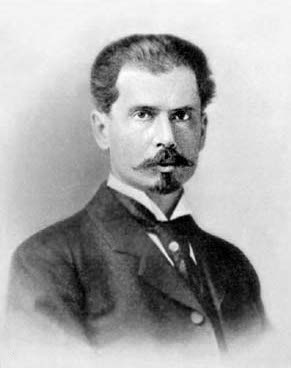
\includegraphics[width=0.26\linewidth]{images/book4/winogradsky.jpg}\hspace{0.05\linewidth}
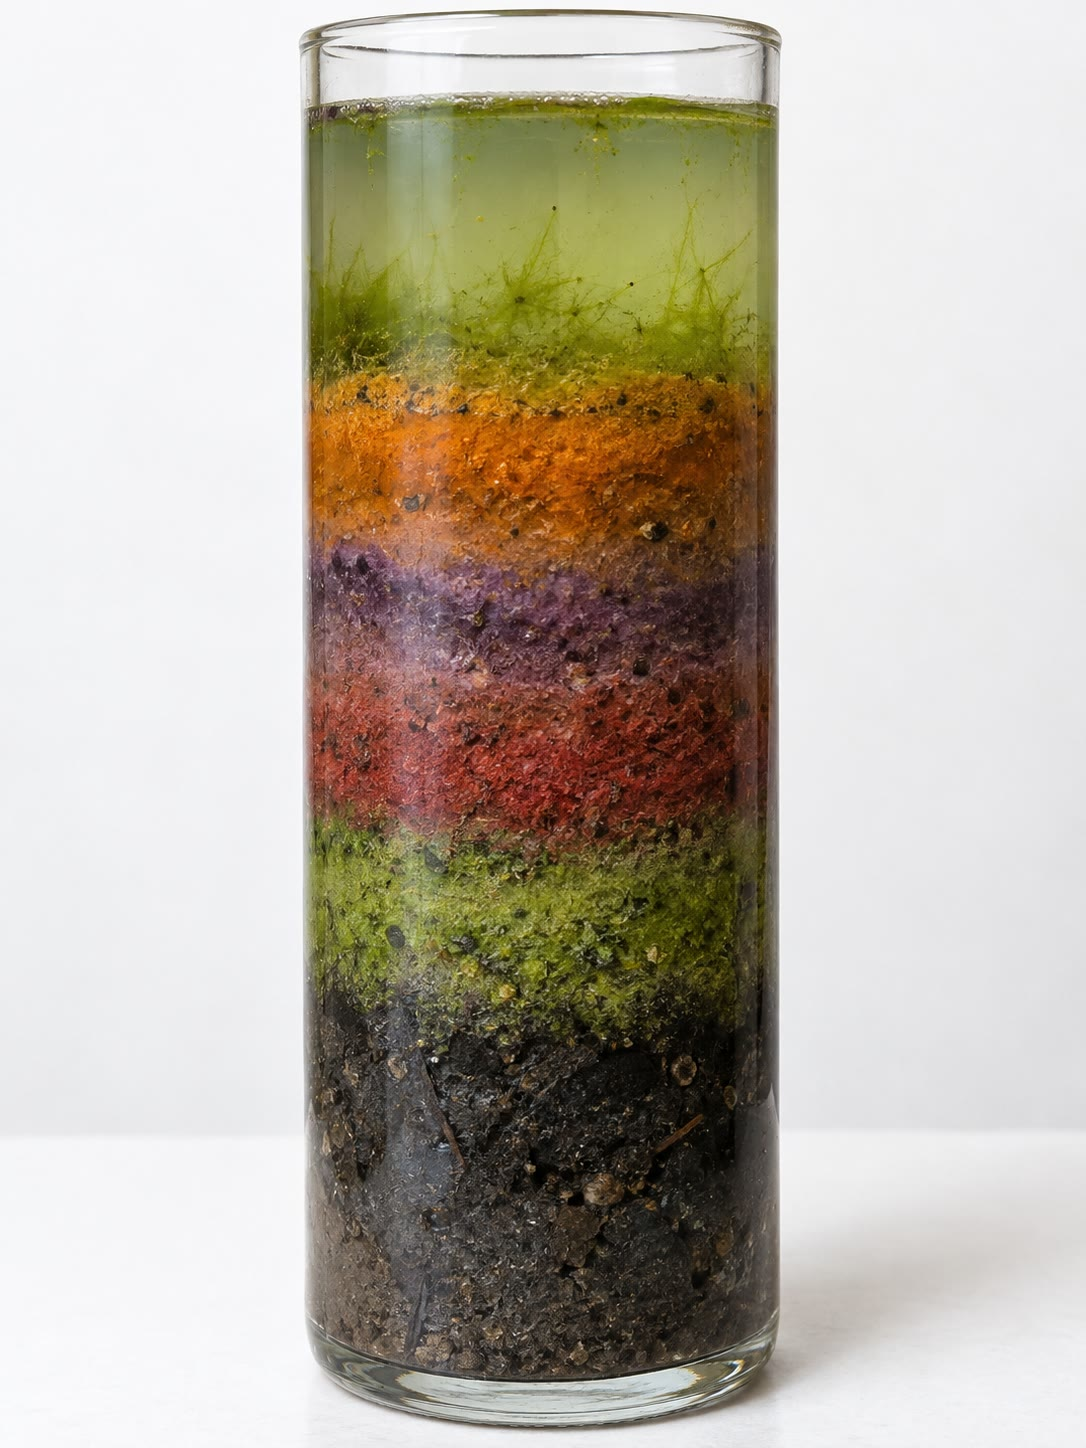
\includegraphics[width=0.30\linewidth]{images/book4/ai/b4-02-winogradsky-column.jpg}

{\small سيرغي فينوغرادسكي، مكتشف التغذي
الكيميائي المعدني، والأسطوانة التي تحمل اسمه: أسطوانة من وحل وماء
تتطبق تحت الضوء إلى نطق من الطحالب، ومؤكسدات الحديد والكبريت،
والبكتيريا الكبريتية الأرجوانية والخضراء، ومرجعات الكبريتات في
الوحل الأسود.}
\end{omfigure}

\begin{definition}[التركيب الضوئي غير المنتج للأكسجين]\label{def:b2:microbial-metabolism:anoxygenic}
\index{تركيب ضوئي غير منتج للأكسجين}
تركّب البكتيريا الأرجوانية والخضراء ضوئيًا بجهاز ضوئي واحد
وبيكتريوكلوروفيل يمتص في الأشعة تحت الحمراء القريبة، مستعملة
$\mathrm{H_2S}$ أو $\mathrm{H_2}$ أو حموضًا عضوية واهبات إلكترون بدل
الماء: فهي تطلق كبريتًا أو كبريتات لا أكسجين قط، وتحتاج إلى ضوء
بأطوال موجة تنفذ عبر الطبقة الخضراء والزراقمية فوقها. ولذلك تنمو
البكتيريا الكبريتية الأرجوانية في النطاق الأرجواني من أسطوانة
فينوغرادسكي، حيث يلتقي الكبريتيد الصاعد من الأسفل بالضوء النازل من
الأعلى؛ وتنمو تحتها البكتيريا الكبريتية الخضراء، وهي أحمل للكبريتيد
وأقنع بالضوء القليل. أما التركيب الضوئي المنتج للأكسجين، بجهازيه
الضوئيين على التوالي، فابتكار متأخر لسلالة واحدة --- الزراقم ---
تعلمت أخذ الإلكترونات من الماء.
\end{definition}

\section{التنفسات اللاهوائية والتخمرات}

\begin{definition}[التنفس اللاهوائي]\label{def:b2:microbial-metabolism:anaerobic}
\index{تنفس لاهوائي}\index{نزع النترتة}\index{إرجاع الكبريتات}\index{توليد الميثان}
\emph{التنفس اللاهوائي} تنفس --- أي سلسلة نقل إلكترونات تضخ
البروتونات وتصنع ATP بالتناضح الكيميائي --- بمتقبل نهائي غير
الأكسجين. \emph{فنازعات النترتة} (\emph{Pseudomonas}،
\emph{Paracoccus}) ترجع النترات إلى نتريت، ثم أكسيد نتريك، ثم أكسيد
نيتروز، وأخيرًا $\mathrm{N_2}$ الذي يفلت إلى الهواء؛ وهي تستعمل
سلسلتها الهوائية مع بضعة إنزيمات مضافة، ولا تنتقل إلى النترات إلا
حين يزول الأكسجين. و\emph{مرجعات الكبريتات}
(\emph{Desulfovibrio}) ترجع الكبريتات إلى كبريتيد، فتسوّد الوحل
بكبريتيد الحديد وتكسبه رائحته. و\emph{مولّدات الميثان}، وهي عتائق،
ترجع $\mathrm{CO_2}$ بالهدروجين $\mathrm{H_2}$ إلى ميثان
($4\mathrm{H_2} + \mathrm{CO_2} \to \mathrm{CH_4} +
2\mathrm{H_2O}$، $\Delta G^{\circ\prime} = \qty{-131}{kJ/mol}$)، أو
تشق الأسيتات إلى ميثان و$\mathrm{CO_2}$؛ ويقتلها الأكسجين، وتعيش في
كروش الأبقار وحقول الأرز والمستنقعات والمطامر، ومنها تطلق غاز
دفيئة هو موضوع \cref{ch:b2:global-change}. وتخدم أكاسيد الحديد
والمنغنيز مجموعات أخرى. وقد عالج مجلد السنة الأولى الأكسجين بوصفه
\emph{المتقبل}؛ أما في معظم تاريخ الأرض، وفي كل رسابة اليوم، فليس
إلا أول سلسلة.
\end{definition}

\begin{proposition}[تعاقب المتقبلات في رسابة]\label{prop:b2:microbial-metabolism:sequence}
بالنزول عبر رسابة مشبعة بالماء، تُستنفد متقبلات الإلكترون بترتيب
الطاقة التي تعطيها: الأكسجين في الميليمترات الأولى، ثم النترات، ثم
أكاسيد المنغنيز والحديد، ثم الكبريتات، وأخيرًا $\mathrm{CO_2}$
(\omterm{def:b2:microbial-metabolism:anaerobic}{توليد الميثان}) في أعمق طبقة لاأكسجينية. والترتيب هو ترتيب البرج:
فعند كل عمق تنمو الكائنات التي تستعمل أفضل متقبل باقٍ أسرع من
غيرها، فتغلب البقية على الواهبات العضوية، وتستنفد متقبلها قبل أن
تتسلم المجموعة التالية. وفي البحر، حيث الكبريتات وفيرة
(\qty{28}{mmol/L})، يكون نطاق الكبريتات سميكًا ولا يبدأ \omterm{def:b2:microbial-metabolism:anaerobic}{توليد
الميثان} إلا على عمق أمتار؛ أما في مستنقع عذب فقير بالكبريتات فيتكون
الميثان تحت السطح مباشرة.
\end{proposition}

\begin{omfigure}
\begin{tikzpicture}[every node/.style={font=\scriptsize}]
  \fill[omDef!8] (0,0) rectangle (4,0.6);
  \node at (2,0.3) {ماء};
  \fill[omExo!35] (0,-0.5) rectangle (4,0);
  \fill[omProp!25] (0,-1.3) rectangle (4,-0.5);
  \fill[omProp!45] (0,-2.0) rectangle (4,-1.3);
  \fill[gray!50] (0,-3.4) rectangle (4,-2.0);
  \fill[black!75] (0,-4.4) rectangle (4,-3.4);
  \draw[thick] (0,0.6) -- (0,-4.4); \draw[thick] (4,0.6) -- (4,-4.4);
  \draw[thick] (0,0) -- (4,0);
  \node[anchor=west, align=left] at (4.2,-0.25) {تنفس بالأكسجين: $\mathrm{O_2 \to H_2O}$ --- \qty{2.9}{MJ} لكل غلوكوز};
  \node[anchor=west, align=left] at (4.2,-0.9) {إرجاع النترات: $\mathrm{NO_3^- \to N_2}$ --- \qty{2.7}{MJ}};
  \node[anchor=west, align=left] at (4.2,-1.65) {إرجاع المنغنيز والحديد: $\mathrm{Fe^{3+} \to Fe^{2+}}$};
  \node[anchor=west, align=left, white] at (0.1,-2.7) {};
  \node[anchor=west, align=left] at (4.2,-2.7) {إرجاع الكبريتات: $\mathrm{SO_4^{2-} \to H_2S}$ --- \qty{0.5}{MJ}};
  \node[anchor=west, align=left] at (4.2,-3.9) {توليد الميثان: $\mathrm{CO_2 \to CH_4}$ --- \qty{0.4}{MJ}};
  \draw[->, thick] (-0.5,0) -- (-0.5,-4.4) node[below] {العمق};
  \node[anchor=east] at (-0.6,-0.25) {mm};
  \node[anchor=east] at (-0.6,-2.7) {cm إلى m};
\end{tikzpicture}

{\small تعاقب متقبلات الإلكترون مع العمق في رسابة، بترتيب الطاقة
التي يعطيها كل منها لكل غلوكوز. وكائنات كل نطاق تغلب التالية على
المادة العضوية حتى يُستنفد متقبلها.}
\end{omfigure}

\begin{definition}[التخمر، مرة أخرى]\label{def:b2:microbial-metabolism:fermentation}
\index{تخمر!جرثومي}
\emph{التخمر} لا يستعمل متقبلًا خارجيًا: فالركيزة العضوية تُشق إلى
ناتج أكثر أكسدة وآخر أكثر إرجاعًا، ولا يُصنع ATP إلا بالفسفرة على
مستوى الركيزة، ويُعاد أكسدة NADH الناتج من التحلل السكري بإرجاع
مستقلَب. فالخمائر تصنع الإيثانول و$\mathrm{CO_2}$؛ والبكتيريا
اللبنية تصنع اللاكتات (اللبن الرائب، ومخلل الملفوف، والعضلات
الموجعة)؛ و\emph{E.~coli} تصنع خليطًا من الحموض والإيثانول
والغازات؛ والمطثيات تصنع البوتيرات والبوتانول والأسيتون؛
والبروبيونيات تصنع البروبيونات و$\mathrm{CO_2}$ اللذين في الجبن
السويسري. والمردود اثنان من ATP لكل غلوكوز في مقابل نحو ثلاثين
بالتنفس، فعلى المخمّر أن يعالج سكرًا أكثر بخمس عشرة مرة للنمو نفسه،
ونواتجه --- حموض وكحول --- تسمّم وسطه: فالتخمرات تحفظ الطعام لأن
المخمّر يجعل الطعام غير صالح للسكنى، حتى لنفسه.
\end{definition}

\begin{example}[التغذي التعاوني: العيش على البقية]\label{ex:b2:microbial-metabolism:syntrophy}
في رسابة لاأكسجينية تترك المخمّرات وراءها الأسيتات والبروبيونات
والبوتيرات و$\mathrm{H_2}$. وأكسدة البروبيونات إلى أسيتات
و$\mathrm{H_2}$ لها طاقة حرة معيارية \emph{موجبة}
(\qty{+76}{kJ/mol}) وهي مستحيلة --- ما لم يستهلك مولّد ميثان مجاور
الهدروجين بسرعة تكوّنه، فيُبقي ضغطه الجزئي دون \qty{1e-4}{atm}،
وعندها يصير التفاعل مولّدًا للطاقة. ولا يستطيع أي من الشريكين النمو
وحده على البروبيونات؛ وهما معًا يحولانه إلى ميثان. وهذا
\emph{النقل البينوعي للهدروجين} هو سبب كون الهضم اللاهوائي دائمًا
عمل جماعة، وسبب وجدان العتيقة وشريكتها البكتيرية ملتصقتين إحداهما
بالأخرى في كثير من الأحيان.
\end{example}

\section{النمو على ركيزة}

\begin{theorem}[قانون مونو]\label{thm:b2:microbial-metabolism:monod}
\index{معادلة مونو}\index{معامل المردود}
جمهرة تنمو على ركيزة محدِّدة واحدة تركيزها $S$ يكون معدل نموها
النوعي
\[
\mu = \mu_{\max}\,\frac{S}{K_s + S}, \qquad \frac{\mathrm{d}X}{\mathrm{d}t} = \mu X,
\]
حيث $X$ تركيز الكتلة الحيوية، و$\mu_{\max}$ المعدل الأقصى (مقلوب
أقصر زمن جيل مقسومًا على $\ln 2$)، و$K_s$ \emph{ثابت نصف الإشباع}،
أي تركيز الركيزة الذي يجري عنده النمو بنصف سرعته --- بضعة
مليغرامات من الغلوكوز في اللتر عند \emph{E.~coli}. وتُستهلك الركيزة
بنسبة النمو، $\mathrm{d}S/\mathrm{d}t =
-\mu X/Y$، حيث $Y$ هو \emph{المردود}: غرامات الكتلة الحيوية لكل غرام
ركيزة، وهو نحو \num{0.5} في النمو الهوائي على السكر و\num{0.1} عند
مخمّر.
\end{theorem}
\begin{proof}[شواهد]
نمّى مونو (1942) \emph{E.~coli} في دفعات على سلسلة من تراكيز
الغلوكوز وقاس المعدل الأسّي لكل منها: فارتفعت المعدلات مع التركيز
ثم أشبعت، على شكل منحني ميكايليس--منتن، وهو ما يُتوقع إذا كان
المعدل تحدده جملة اقتناء قابلة للإشباع. والقانون تجريبي --- فللخلية
آلاف الإنزيمات لا إنزيم واحد --- لكنه يوافق كل مزرعة محدودة الركيزة
تقريبًا، وهو أساس تقانة التخمير وهندسة معالجة المياه المستعملة.
\end{proof}

\begin{theorem}[المزرعة الكيميائية المستقرة]\label{thm:b2:microbial-metabolism:chemostat}
\index{مزرعة كيميائية مستقرة}\index{معدل التمديد}
\emph{\omterm{thm:b2:microbial-metabolism:chemostat}{المزرعة الكيميائية المستقرة}} وعاء حجمه $V$ يُغذَّى بوسط طازج
(ركيزته $S_{\text{الوارد}}$) بتدفق $F$ ويُفرَّغ بالتدفق نفسه، فيكون
\emph{\omterm{thm:b2:microbial-metabolism:chemostat}{معدل التمديد}} $D = F/V$. وتخضع الكتلة الحيوية والركيزة إلى
\[
\frac{\mathrm{d}X}{\mathrm{d}t} = (\mu - D)\,X, \qquad
\frac{\mathrm{d}S}{\mathrm{d}t} = D\,(S_{\text{الوارد}} - S) - \frac{\mu X}{Y}.
\]
وفي الحالة المستقرة $\mu = D$: أي إن المزرعة تنمو بالسرعة نفسها
التي تُغسل بها، مهما كان $D$ دون قيمة حرجة، فيضبط المشغّل معدل
النمو بإدارة المضخة. أما الركيزة والكتلة الحيوية في الحالة
المستقرة فهما
\[
S^* = \frac{K_s\,D}{\mu_{\max} - D}, \qquad X^* = Y\,(S_{\text{الوارد}} - S^*),
\]
وفوق معدل \emph{الغسل} $D_c = \mu_{\max}
S_{\text{الوارد}}/(K_s + S_{\text{الوارد}})$ لا تستطيع أي جمهرة الصمود.
\end{theorem}
\begin{proof}
بوضع $\mathrm{d}X/\mathrm{d}t = 0$ مع $X \neq 0$ نجد $\mu = D$؛
وبقلب قانون مونو، $D(K_s + S^*) = \mu_{\max} S^*$، ومنه $S^* =
K_s D/(\mu_{\max} - D)$. وبوضع $\mathrm{d}S/\mathrm{d}t = 0$
وتعويض $\mu$ بالمقدار $D$: $D(S_{\text{الوارد}} - S^*) = DX^*/Y$، ومنه
$X^*$. ولا يوجد الحل إلا ما دام $S^* < S_{\text{الوارد}}$، أي
$D < \mu_{\max} S_{\text{الوارد}}/(K_s + S_{\text{الوارد}})$؛ وبعد ذلك
يكون $\mu < D$ من أجل كل $S \le S_{\text{الوارد}}$ ويؤول $X$ إلى الصفر.
والحالة المستقرة مستقرة: فإذا ارتفع $X$ هبط $S$، فهبط $\mu$ دون
$D$، فأُعيد $X$ بالغسل إلى أسفل.
\end{proof}

\begin{omfigure}
\begin{minipage}[b]{0.48\linewidth}\centering
\begin{tikzpicture}
\begin{axis}[
  width=0.94\linewidth, height=5.4cm,
  axis x line=bottom, axis y line=left,
  xmin=0, xmax=0.5, ymin=0, ymax=1.1,
  xlabel={$S$ (\unit{g/L})}, ylabel={$\mu$ (\unit{h^{-1}})},
  xlabel style={font=\small, at={(axis description cs:0.5,-0.14)}, anchor=north},
  ylabel style={font=\small},
  tick label style={font=\small}, xtick={0,0.1,0.2,0.3,0.4,0.5}, ytick={0,0.5,1},
  clip=false,
]
\addplot[very thick, omDef, domain=0:0.5, samples=100] {x/(0.02+x)};
\draw[dashed, gray] (axis cs:0,1) -- (axis cs:0.5,1); \node[font=\scriptsize, anchor=south east] at (axis cs:0.5,1) {$\mu_{\max}$};
\draw[dashed, gray] (axis cs:0,0.5) -- (axis cs:0.02,0.5) -- (axis cs:0.02,0); \node[font=\scriptsize, anchor=north west] at (axis cs:0.02,-0.02) {$K_s$};
\end{axis}
\end{tikzpicture}
\end{minipage}\hfill
\begin{minipage}[b]{0.5\linewidth}\centering
\begin{tikzpicture}
\begin{axis}[
  width=0.94\linewidth, height=5.4cm,
  axis x line=bottom, axis y line=left,
  xmin=0, xmax=1.1, ymin=0, ymax=2.2,
  xlabel={معدل التمديد $D$ (\unit{h^{-1}})}, ylabel={\unit{g/L}},
  xlabel style={font=\small, at={(axis description cs:0.5,-0.14)}, anchor=north},
  ylabel style={font=\small},
  tick label style={font=\small}, xtick={0,0.5,1}, ytick={0,1,2},
  legend style={font=\scriptsize, at={(0.05,0.62)}, anchor=west, draw=none},
  clip=false,
]
\addplot[very thick, omDef, domain=0:0.99, samples=200] {0.5*(2 - 0.02*x/(1-x))};
\addlegendentry{الكتلة الحيوية $X^*$}
\addplot[very thick, omThm, domain=0:0.99, samples=200] {0.02*x/(1-x)};
\addlegendentry{الركيزة $S^*$}
\addplot[thick, omProp, dashed, domain=0:0.99, samples=200] {x*0.5*(2 - 0.02*x/(1-x))};
\addlegendentry{الإنتاج $D X^*$}
\draw[dashed, gray] (axis cs:0.99,0) -- (axis cs:0.99,2.1); \node[font=\scriptsize, anchor=south, align=center] at (axis cs:0.9,2.1) {الغسل};
\end{axis}
\end{tikzpicture}
\end{minipage}

{\small على اليمين: قانون مونو مع $\mu_{\max} = \qty{1}{h^{-1}}$
و$K_s = \qty{0.02}{g/L}$. وعلى اليسار: المزرعة المستقرة المغذّاة
بمقدار \qty{2}{g/L} من الركيزة ($Y = 0.5$): تبقى الكتلة الحيوية شبه
ثابتة والركيزة المتبقية شبه معدومة حتى معدل الغسل، وقربه تنفذ
الركيزة وتنهار الجمهرة؛ وإنتاج الكتلة الحيوية في الساعة أعظم ما
يكون قبيله.}
\end{omfigure}

\begin{omfigure}
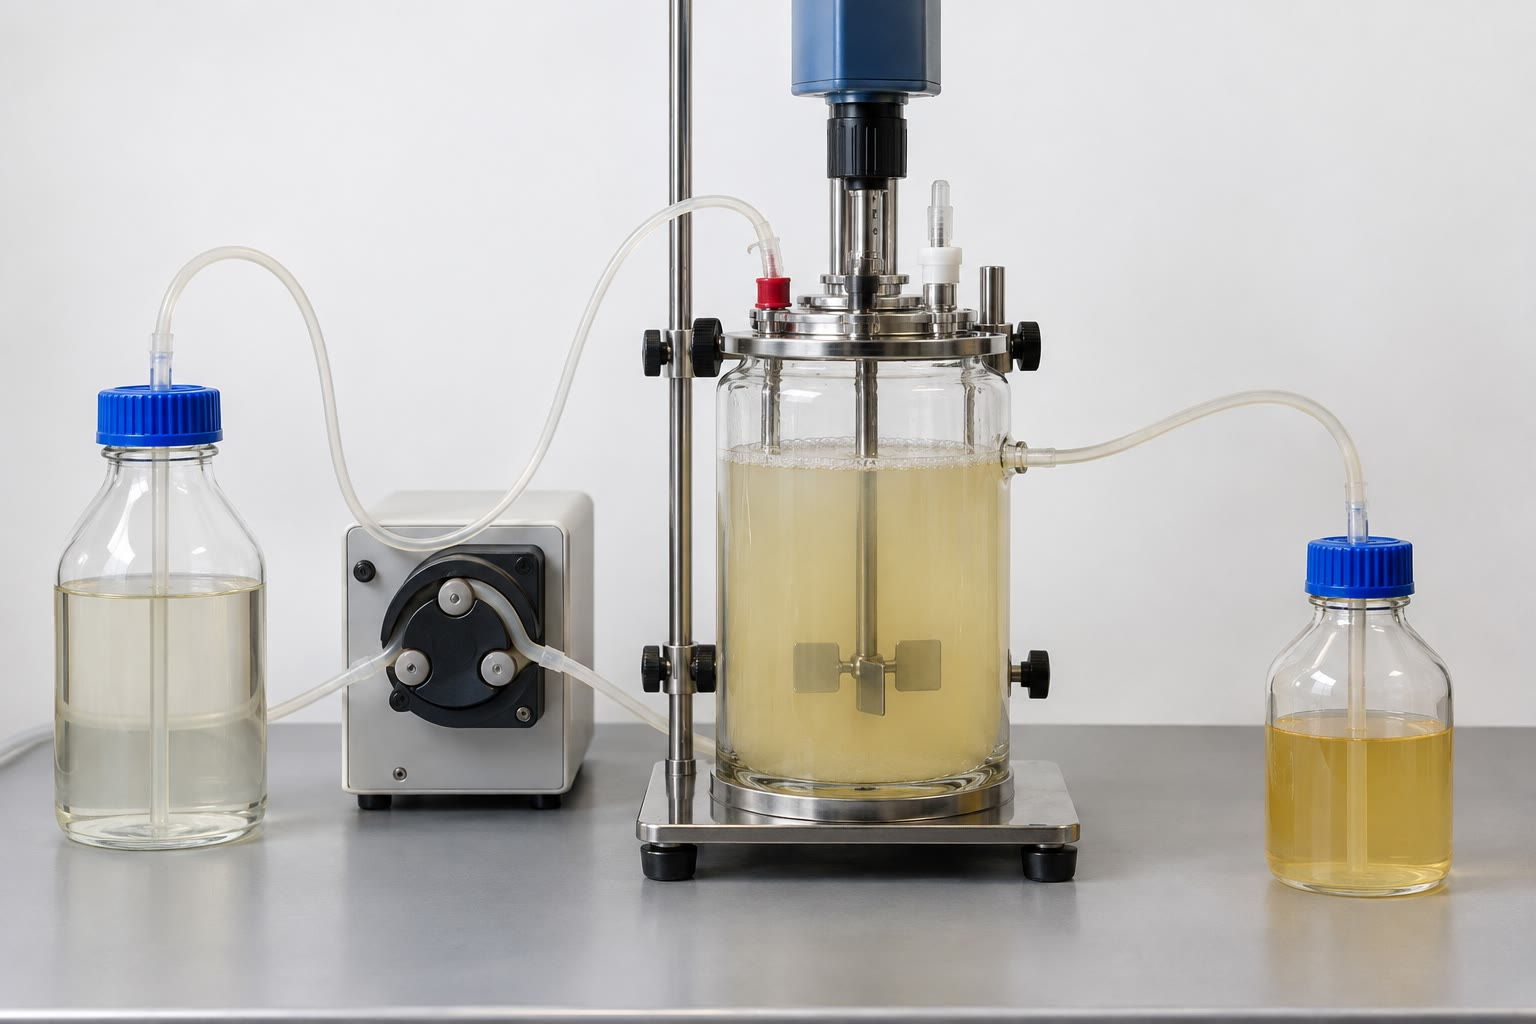
\includegraphics[width=0.6\linewidth]{images/book4/ai/b4-02-chemostat.jpg}

{\small \omterm{thm:b2:microbial-metabolism:chemostat}{مزرعة كيميائية مستقرة} مخبرية: وسط طازج يُضخ من الخزان على
اليمين، ومزرعة تفيض إلى اليسار؛ والمضخة هي التي تضبط معدل النمو.}
\end{omfigure}

\begin{example}[قراءة مزرعة مستقرة]\label{ex:b2:microbial-metabolism:chemostat}
مع $\mu_{\max} = \qty{1.0}{h^{-1}}$، و$K_s = \qty{0.02}{g/L}$،
و$S_{\text{الوارد}} = \qty{2}{g/L}$، و$Y = 0.5$، عند $D =
\qty{0.5}{h^{-1}}$: يكون $S^* = 0.02\times 0.5/0.5 = \qty{0.02}{g/L}$
و$X^* = 0.5\times 1.98 = \qty{0.99}{g/L}$؛ فتترك المزرعة
\qty{1}{\%} من السكر دون استعمال. ومعدل الغسل هو $1.0\times
2/2.02 = \qty{0.99}{h^{-1}}$. ويعمل الهاضم أو الأمعاء بالمبدأ نفسه:
فالقولون البشري، الذي يُغذَّى ثلاث مرات في اليوم ويُفرَّغ مرة، يبقي
بكتيرياه عند معدل تمديد قريب من \qty{0.04}{h^{-1}}، وكل نوع لا
يستطيع التضاعف خلال يوم يُغسل خارجًا --- ما لم يتشبث بالجدار.
\end{example}

\section{الأغشية الحيوية}

\begin{definition}[الغشاء الحيوي]\label{def:b2:microbial-metabolism:biofilm}
\index{غشاء حيوي}\index{حشوة خارج خلوية!بكتيرية}
\emph{الغشاء الحيوي} جماعة من الكائنات المجهرية ملتصقة بسطح ومغروسة
في \emph{حشوة} من عديدات السكريد والبروتينات وDNA خارج خلوي تنتجها
بنفسها. ويتكون على مراحل: \emph{التصاق} عكوس لخلايا مفردة (بالأسواط
والأهلاب)، ثم التصاق لاعكوس ونمو \emph{مستعمرات مجهرية}، ثم
\emph{نضج} إلى غشاء مبنيّ فيه أبراج وقنوات ماء، ثم \emph{تشتت}
لخلايا تسبح بعيدًا لتبذر سطوحًا جديدة. والحشوة تمسك الماء
والمغذيات، وتحمي الخلايا من الجفاف والراعيات والصادات والخلايا
المناعية، وتقيم تدرجات كيميائية تجعل الغشاء منظرًا من المساكن
البيئية. وهكذا تعيش معظم بكتيريا الأرض: على صخور الجداول، وعلى
الجذور، وعلى الأسنان (اللويحة السنية)، وعلى القثاطر والغرسات، وفي
رئتي مريض التليف الكيسي، وعلى هياكل السفن وفي الأنابيب.
\end{definition}

\begin{omfigure}
\begin{tikzpicture}[every node/.style={font=\scriptsize}]
  \fill[gray!35] (0,0) rectangle (13.6,0.35);
  \node at (6.8,0.17) {السطح};
  % stage 1 attachment
  \foreach \p in {(0.6,0.55),(1.4,0.55)} \draw[thick, omDef, fill=omDef!30] \p ellipse (0.22 and 0.1);
  \draw[thick, omDef, fill=omDef!30] (1.0,1.6) ellipse (0.22 and 0.1);
  \draw[->, omDef] (1.0,1.45) -- (1.0,0.75);
  \node[below, align=center] at (1.1,-0.05) {1. التصاق};
  % stage 2 microcolony
  \begin{scope}[xshift=3.4cm]
    \fill[omExo!25] (0.15,0.35) .. controls (0.1,1.1) and (1.5,1.1) .. (1.45,0.35);
    \foreach \p in {(0.45,0.5),(0.8,0.5),(1.15,0.5),(0.6,0.75),(0.95,0.75),(0.8,0.95)} \draw[thick, omDef, fill=omDef!30] \p ellipse (0.18 and 0.09);
    \node[below, align=center] at (0.8,-0.05) {2. مستعمرة مجهرية،\\وإفراز الحشوة};
  \end{scope}
  % stage 3 mature with channels
  \begin{scope}[xshift=6.8cm]
    \fill[omExo!25] (0.0,0.35) .. controls (0.2,1.9) and (0.9,2.2) .. (1.1,1.5) .. controls (1.2,0.9) and (1.4,0.6) .. (1.5,0.35);
    \fill[omExo!25] (1.7,0.35) .. controls (1.6,1.5) and (2.6,2.3) .. (2.9,1.2) .. controls (3.0,0.8) and (3.1,0.5) .. (3.2,0.35);
    \foreach \p in {(0.35,0.55),(0.7,0.55),(0.5,0.85),(0.8,1.15),(0.55,1.45),(2.0,0.6),(2.4,0.6),(2.2,0.9),(2.5,1.25),(2.3,1.6),(2.6,1.9),(2.1,1.3)} \draw[thick, omDef, fill=omDef!30] \p ellipse (0.16 and 0.08);
    \draw[<->, omThm, thick] (1.6,0.5) -- (1.6,1.6);
    \node[omThm, anchor=south] at (1.6,2.45) {قناة ماء};
    \node[below, align=center] at (1.6,-0.05) {3. غشاء ناضج: أبراج،\\وقنوات، وتدرجات};
  \end{scope}
  % stage 4 dispersal
  \begin{scope}[xshift=11.2cm]
    \fill[omExo!25] (0.0,0.35) .. controls (0.1,1.5) and (1.0,1.6) .. (1.1,0.35);
    \foreach \p in {(0.3,0.55),(0.65,0.55),(0.5,0.85)} \draw[thick, omDef, fill=omDef!30] \p ellipse (0.16 and 0.08);
    \foreach \p/\a in {(1.4,1.5)/40,(1.9,1.1)/10,(1.6,2.0)/70} \draw[thick, omDef, fill=omDef!30, rotate around={\a:\p}] \p ellipse (0.16 and 0.08);
    \draw[->, omDef] (1.0,1.0) -- (1.35,1.35);
    \node[below, align=center] at (1.0,-0.05) {4. تشتت};
  \end{scope}
\end{tikzpicture}

{\small دورة حياة \omterm{def:b2:microbial-metabolism:biofilm}{الغشاء الحيوي}: تلتصق خلايا مفردة، فتنمو إلى
مستعمرات مجهرية تفرز حشوة (بالرمادي)، ثم تنضج إلى غشاء مبنيّ فيه
أبراج وقنوات ماء، ويطلق خلايا سابحة تستعمر سطوحًا جديدة.}
\end{omfigure}

\begin{omfigure}
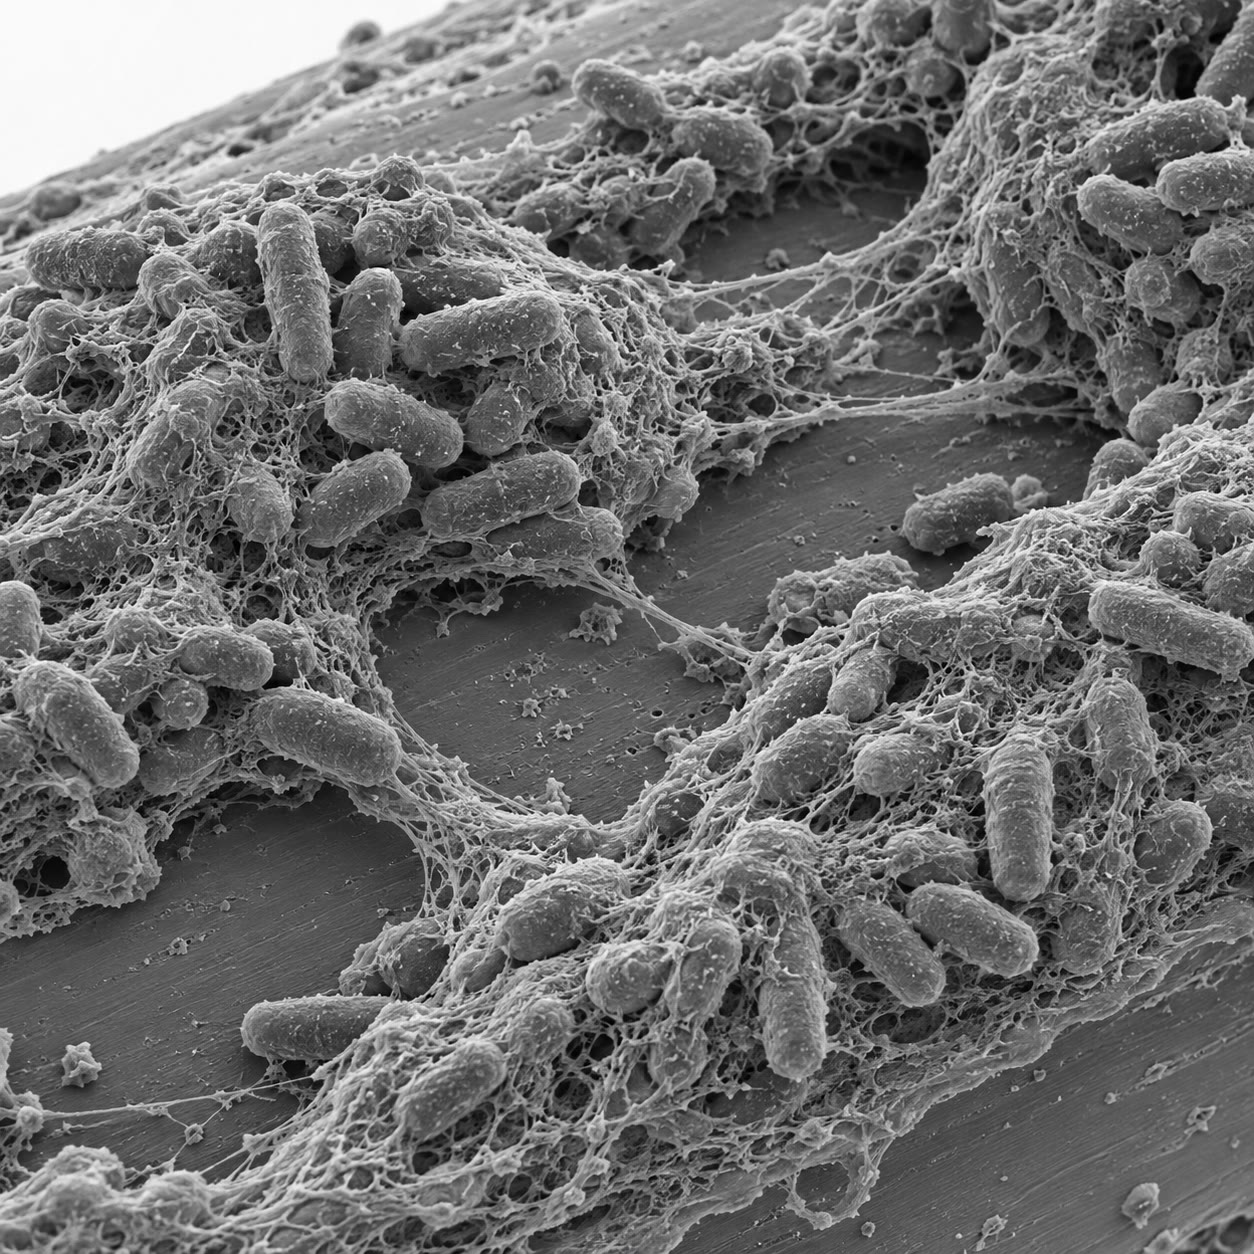
\includegraphics[width=0.46\linewidth]{images/book4/ai/b4-02-biofilm-sem.jpg}

{\small \omterm{def:b2:microbial-metabolism:biofilm}{غشاء حيوي} على قثطار، بالمجهر الإلكتروني الماسح: بكتيريا
عصوية مغروسة في الحشوة الليفية التي أفرزتها، وبينها قنوات مفتوحة
بين العناقيد.}
\end{omfigure}

\begin{theorem}[التدرجات داخل غشاء حيوي]\label{thm:b2:microbial-metabolism:gradient}
\index{عمق نفاذ الأكسجين}
في غشاء ثخنه $L$ تستهلك خلاياه الأكسجين بمعدل حجمي ثابت $q$، مع
إبقاء التركيز عند $c_0$ على السطح ولا تدفق عبر الحامل، يكون مَنْحى
الأكسجين في الحالة المستقرة قطعًا مكافئًا، وإذا كان الغشاء سميكًا
بما يكفي لينفد الأكسجين، نفد عند \emph{عمق النفاذ}
\[
L_p = \sqrt{\frac{2 D_e\, c_0}{q}},
\]
حيث $D_e$ معامل الانتشار الفعلي في الحشوة. فمع
$D_e = \qty{1.5e-9}{m^2/s}$، و$c_0 = \qty{0.25}{mol/m^3}$، و$q
= \qty{0.17}{mol/m^3/s}$ (غشاء كثيف من خلايا متنفسة)، يكون $L_p
\approx \qty{66}{\micro m}$: أي إن \omterm{def:b2:microbial-metabolism:biofilm}{الغشاء الحيوي} دون عُشر المليمتر
لاأكسجيني، وتعيش نازعات النترتة والمخمّرات ومرجعات الكبريتات تحت
سقف من الهوائيات.
\end{theorem}
\begin{proof}
ليكن $x$ العمق تحت السطح. في الحالة المستقرة لا يتغير التدفق
الانتشاري $-D_e\,\mathrm{d}c/\mathrm{d}x$ مع العمق إلا بالاستهلاك:
$D_e\,\mathrm{d}^2c/\mathrm{d}x^2 = q$. وبالمكاملة مرتين،
$c = c_0 + a x + q x^2/2D_e$. وإذا انعدم الأكسجين عند العمق $L_p$
بتدفق معدوم هناك (إذ لا يأتي شيء من الأسفل)، كان $c(L_p) = 0$
و$c'(L_p) = 0$: فالثانية تعطي $a = -qL_p/D_e$، والأولى تعطي عندئذ
$c_0 - qL_p^2/D_e + qL_p^2/2D_e = 0$، أي
$L_p^2 = 2D_e c_0/q$. والمنحى هو $c = (q/2D_e)(L_p - x)^2$.
\end{proof}

\begin{omfigure}
\begin{tikzpicture}
\begin{axis}[
  width=0.78\linewidth, height=5.6cm,
  axis x line=bottom, axis y line=left,
  xmin=0, xmax=120, ymin=0, ymax=0.28,
  xlabel={العمق في الغشاء (\unit{\micro m})}, ylabel={$\mathrm{O_2}$ (\unit{mol/m^3})},
  xlabel style={font=\small, at={(axis description cs:0.5,-0.14)}, anchor=north},
  ylabel style={font=\small},
  tick label style={font=\small}, xtick={0,20,40,60,80,100,120}, ytick={0,0.1,0.2},
  clip=false,
]
\addplot[very thick, omDef, domain=0:66, samples=60] {0.25*(1-x/66)^2};
\addplot[very thick, omDef, domain=66:120, samples=2] {0};
\fill[omThm!12] (axis cs:66,0) rectangle (axis cs:120,0.28);
\node[font=\scriptsize, anchor=north, align=center] at (axis cs:93,0.27) {النطاق اللاأكسجيني:\\نازعات النترتة، والمخمّرات،\\ومرجعات الكبريتات};
\draw[dashed, gray] (axis cs:66,0) -- (axis cs:66,0.28); \node[font=\scriptsize, anchor=south] at (axis cs:66,0.28) {$L_p$};
\node[font=\scriptsize, anchor=west] at (axis cs:24,0.18) {النطاق الهوائي};
\end{axis}
\end{tikzpicture}

{\small الأكسجين داخل \omterm{def:b2:microbial-metabolism:biofilm}{غشاء حيوي} متنفس: هبوط قطعي مكافئ من قيمة
الحجم على السطح إلى الصفر عند عمق النفاذ، وهو \qty{66}{\micro m}
عند أرقام المبرهنة. وكل ما هو أعمق لاأكسجيني.}
\end{omfigure}

\begin{proposition}[استشعار النصاب]\label{prop:b2:microbial-metabolism:quorum}
\index{استشعار النصاب}\index{محرّض ذاتي}
البكتيريا تعدّ نفسها. فكل خلية تفرز جزيئة إشارة صغيرة،
\emph{محرّضًا ذاتيًا} (لاكتونات أسيل-هوموسيرين عند سلبيات الغرام،
وببتيدات قصيرة عند إيجابياتها)، بمعدل ثابت منخفض. وفي معلق مخفف
تنتشر الإشارة بعيدًا؛ أما في جمهرة كثيفة أو \omterm{def:b2:microbial-metabolism:biofilm}{غشاء حيوي} فتتراكم، وفوق
تركيز عتبي ترتبط بمستقبل يشغّل طائفة من المورّثات --- منها مورّثة
\omterm{prop:b2:microbial-metabolism:quorum}{المحرّض الذاتي} نفسه، ومن هنا اسمه. والمورّثات التي تُضبط هكذا هي
التي لا تجدي إلا حين تعمل خلايا كثيرة معًا: التلألؤ، وإفراز
الإنزيمات الهاضمة والذيفانات، وإنتاج الحشوة، وفوعة الممرضات التي
عليها أن تغمر المضيف دفعة واحدة لا أن تنبهه خلية خلية.
\end{proposition}
\begin{proof}[شواهد]
وجد نيلسون وبلات وهاستينغز (1970) أن البكتيريا البحرية
\emph{Vibrio fischeri}، التي تضيء عضو حبّار، مظلمة في المزرعة
المخففة ولا تتوهج إلا فوق نحو $10^{7}$ خلية في المليلتر؛ وأن وسطًا
خاليًا من الخلايا مأخوذًا من مزرعة كثيفة متوهجة يجعل مزرعة مخففة
تتوهج في الحال. فالوسط كان يحوي الإشارة؛ وحُدّدت بنيتها، وهي لاكتون
أسيل-هوموسيرين، سنة 1981، والطافرات العاجزة عن صنعها لا تتوهج أبدًا
مهما كثفت.
\end{proof}

\begin{example}[لماذا ينجو غشاء حيوي من الصادات]\label{ex:b2:microbial-metabolism:tolerance}
تنجو خلايا \omterm{def:b2:microbial-metabolism:biofilm}{الغشاء الحيوي} من تراكيز صادّ تفوق بمئة إلى ألف مرة تلك
التي تقتل السلالة نفسها في معلق، دون أي مورّثة مقاومة. فالحشوة تبطئ
انتشار الدواء وتربط بعضه؛ والتدرجات تترك الخلايا العميقة جائعة
ولاأكسجينية ولا تكاد تنمو، ومعظم الصادات لا تقتل إلا الخلايا
النامية (البنسلينات تحتاج إلى اصطناع الجدار، والأمينوغليكوزيدات
تحتاج إلى نقل فعال)؛ وقليل من \emph{الخلايا المثابرة} ساكن تمامًا
ويعيد إنماء الغشاء حين يتوقف العلاج. ولذلك يُعالَج خمج مزمن على
غرسة عادةً بنزع الغرسة.
\end{example}

\section{الجماعات الجرثومية}

\begin{example}[أسطوانة فينوغرادسكي، مشروحة]\label{ex:b2:microbial-metabolism:column}
يدخل الضوء والهواء من الأعلى؛ وتأتي المادة العضوية والكبريتات من
الوحل. فتنمو الزراقم والطحالب في الأعلى وتطلق الأكسجين. وتحتها
تستنفد غير ذاتيات التغذي الأكسجين على المادة العضوية، ثم النترات؛
وأعمق منها ترجع مرجعات الكبريتات الكبريتات إلى كبريتيد ينتشر صاعدًا
فيسوّد الوحل بكبريتيد الحديد. وحيث يلتقي الكبريتيد الصاعد بالضوء
النازل، تؤكسده البكتيريا الكبريتية الأرجوانية ضوئيًا (النطاق
الأرجواني)، وتحتها البكتيريا الكبريتية الخضراء؛ وحيث يلتقي
الكبريتيد بالأكسجين، في الظلام، تكسب مؤكسدات الكبريت عديمة اللون
مثل \emph{Beggiatoa} عيشها بالتغذي الكيميائي المعدني (الحجاب
الأبيض)؛ وحيث يلتقي الحديد المرجع بالأكسجين، تترك مؤكسدات الحديد
نطاقًا صدئًا. فالكبريت يدور بين كبريتيد وكبريتات داخل الأسطوانة؛
والكربون يدور بين $\mathrm{CO_2}$ ومادة عضوية؛ ولا يدخل إلا الضوء
ولا يخرج إلا الحرارة. فهي نظام بيئي مغلق بميزان طاقة مفتوح، ونموذج
مصغر لقاع المحيط.
\end{example}

\begin{omfigure}
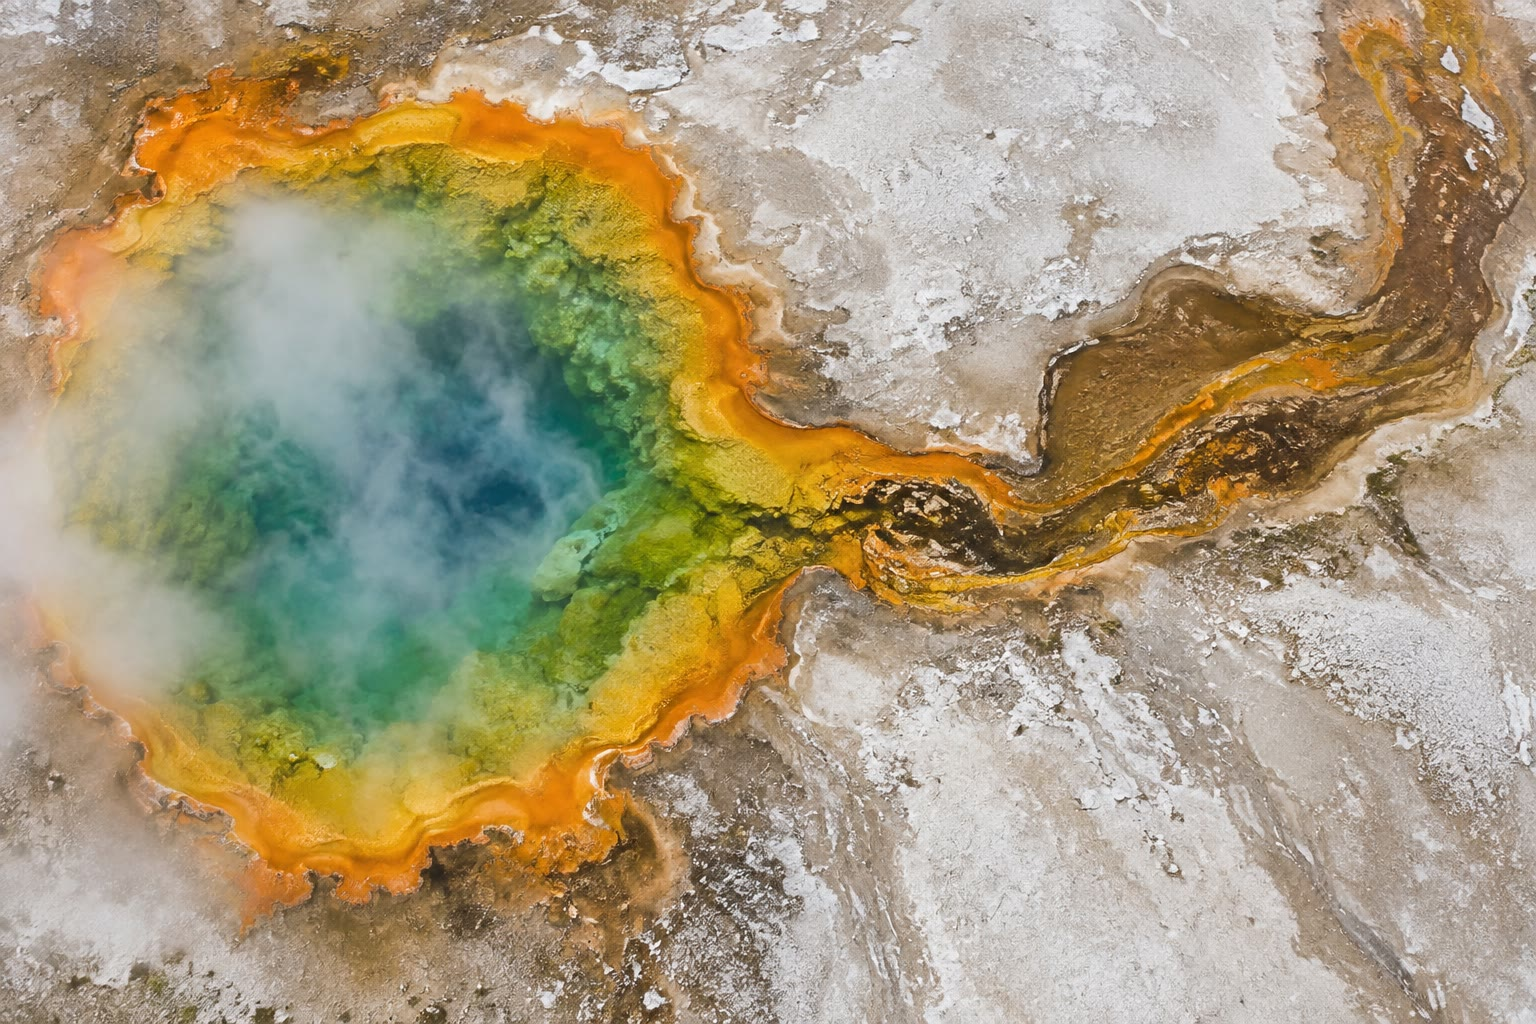
\includegraphics[width=0.62\linewidth]{images/book4/ai/b4-02-hot-spring-mats.jpg}

{\small حصر جرثومية حول ينبوع حار: كل لون جمهرة تعيش عند درجة
حرارة نطاقها وكيميائه --- زراقم محبة للحرارة وبكتيريا خضراء في
المصبّ الأبرد، \omterm{def:b2:microbial-metabolism:trophic}{ومتغذيات كيميائية معدنية} عديمة اللون في أحرّ الماء.}
\end{omfigure}

\begin{remark}[الحصر الجرثومية والأرض المبكرة]\label{rem:b2:microbial-metabolism:mats}
حول الينابيع الحارة وعلى السهول المدّية، تحشر حصر جرثومية مطبقة
ثخنها بضعة مليمترات الأسطوانة كلها في ثخن يستطيع الضوء عبوره:
زراقم في الأعلى، وبكتيريا أرجوانية تحتها، ومرجعات كبريتات في
القاعدة، وكل طبقة تستهلك ما تنتجه التي فوقها، والحصيرة تهاجر صاعدة
عبر الرسابة التي تحبسها. والحصر المتحجرة --- الستروماتوليت --- هي
أقدم دليل على الحياة، وعمرها \num{3.5} مليار سنة. فطوال ملياري سنة،
قبل النباتات والحيوانات، كان المحيط الحيوي هذه الحصر والعوالق
فوقها، وهي التي ملأت الهواء بالأكسجين
(\cref{ch:b2:biogeochemical-cycles}).
\end{remark}

\section{تمارين}

\begin{exercise}[$\star$]\label{exo:b2:microbial-metabolism:1}
صنّف بحسب مصدر الطاقة ومصدر الإلكترونات ومصدر الكربون: زُراق؛
و\emph{Nitrosomonas}؛ و\emph{E.~coli} على الغلوكوز؛ وبكتيريا
أرجوانية غير كبريتية تنمو في الضوء على السكسينات؛
و\emph{Thiobacillus} على $\mathrm{H_2S}$ في الظلام.
\end{exercise}

\begin{exercise}[$\star$]\label{exo:b2:microbial-metabolism:2}
اذكر متقبلات الإلكترون في التنفس بترتيب تناقص المردود الطاقي، وقل
أين يُستعمل كل منها في رسابة.
\end{exercise}

\begin{exercise}[$\star$]\label{exo:b2:microbial-metabolism:3}
وازن أكسدة الغلوكوز إلى $\mathrm{CO_2}$ بنترات مرجعة إلى
$\mathrm{N_2}$ (في وسط حمضي، والماء هو الناتج الآخر). فكم شاردة
نترات لكل غلوكوز؟
\end{exercise}

\begin{exercise}[$\star$]\label{exo:b2:microbial-metabolism:4}
عرّف \omterm{def:b2:microbial-metabolism:biofilm}{الغشاء الحيوي} وسمِّ مراحله الأربع. واذكر ثلاثة مواضع تهم فيها
الأغشية الحيوية صحة الإنسان أو الصناعة.
\end{exercise}

\begin{exercise}[$\star\star$]\label{exo:b2:microbial-metabolism:5}
احسب $\Delta G^{\circ\prime}$ من أجل $4\mathrm{H_2} + \mathrm{CO_2}
\to \mathrm{CH_4} + 2\mathrm{H_2O}$ انطلاقًا من الكمونين
$\mathrm{2H^+/H_2}$ (\qty{-0.42}{V}) و$\mathrm{CO_2/CH_4}$
(\qty{-0.24}{V}). وكم جزيء ATP (عند \qty{50}{kJ/mol}) يستطيع مولّد
الميثان صنعه على الأكثر لكل $\mathrm{H_2}$؟ وعلّق على معدل نموه.
\end{exercise}

\begin{exercise}[$\star\star$]\label{exo:b2:microbial-metabolism:6}
بكتيريا لها $\mu_{\max} = \qty{1.2}{h^{-1}}$ و$K_s =
\qty{5}{mg/L}$ من الغلوكوز. احسب $\mu$ \omterm{def:b2:unicellular-diversity:division}{وزمن الجيل} عند 1 و5
و\qty{50}{mg/L}. وعند أي تركيز تنمو بنسبة \qty{90}{\%} من أقصاها؟
\end{exercise}

\begin{exercise}[$\star\star$]\label{exo:b2:microbial-metabolism:7}
مزرعة مستقرة لها $\mu_{\max} = \qty{0.8}{h^{-1}}$، و$K_s =
\qty{0.05}{g/L}$، و$S_{\text{الوارد}} = \qty{5}{g/L}$، و$Y = 0.4$، تعمل عند
$D = \qty{0.4}{h^{-1}}$. احسب $S^*$ و$X^*$ وإنتاج الكتلة الحيوية
لكل لتر في الساعة ومعدل الغسل.
\end{exercise}

\begin{exercise}[$\star\star$]\label{exo:b2:microbial-metabolism:8}
أكسدة $\mathrm{NH_4^+}$ واحد إلى نتريت تعطي \qty{275}{kJ}؛ ويقبض
المُنَترِت ربعها بصيغة ATP (\qty{50}{kJ/mol})، ويكلف تثبيت
$\mathrm{CO_2}$ واحد في الكتلة الحيوية ما يعادل 12 جزيء ATP. فكم
شاردة أمونيوم عليه أن يؤكسد لكل كربون مثبَّت؟ ولماذا يكون مردود
المُنَترِت ضئيلًا هكذا بالقياس إلى مردود غير ذاتي التغذي؟
\end{exercise}

\begin{exercise}[$\star\star$]\label{exo:b2:microbial-metabolism:9}
احسب \omterm{thm:b2:microbial-metabolism:gradient}{عمق نفاذ الأكسجين} في \omterm{def:b2:microbial-metabolism:biofilm}{غشاء حيوي} له $D_e =
\qty{1.2e-9}{m^2/s}$، و$c_0 = \qty{0.20}{mol/m^3}$، و$q =
\qty{0.5}{mol/m^3/s}$. وماذا يحدث للمقدار $L_p$ إذا تضاعف أكسجين الحجم؟
وإذا تنفست الخلايا أسرع بأربع مرات؟
\end{exercise}

\begin{exercise}[$\star\star\star$]\label{exo:b2:microbial-metabolism:10}
تنبّأ بنطق أسطوانة فينوغرادسكي من الأعلى إلى الأسفل، مسمّيًا
استقلاب كل نطاق، واشرح (أ) لماذا يتكون النطاق الأرجواني حيث يتكون،
(ب) ولماذا يسودّ الوحل، (ج) وبأي معنى تكون الأسطوانة جملة مغلقة
وبأي معنى تكون مفتوحة.
\end{exercise}

\begin{exercise}[$\star\star\star$]\label{exo:b2:microbial-metabolism:11}
كل خلية من جمهرة كثافتها $n$ (خلية في اللتر) تفرز محرّضًا ذاتيًا
بمعدل $p = 5$ جزيئات في الثانية؛ وتتحلل الجزيئة بمعدل
$k = \qty{5e-4}{s^{-1}}$. اكتب تركيز الحالة المستقرة $A^*$ بدلالة
$n$. ويشتغل المستقبل عند $A_c = \qty{10}{nmol/L}$: احسب الكثافة
العتبية بالخلايا في المليلتر. وقارنها بمزرعة كثيفة ($10^{9}$ في
المليلتر) وبماء البحر ($10^{5}$ في المليلتر)، واشرح لماذا يبلغ \omterm{def:b2:microbial-metabolism:biofilm}{غشاء
حيوي} النصاب في حجم لا يبلغه فيه معلق أبدًا.
\end{exercise}

\begin{exercise}[$\star\star\star$]\label{exo:b2:microbial-metabolism:12}
«بدائيات النوى تدير كيمياء الكوكب.» ناقش هذا بثلاث عمليات من هذا
الفصل لا يستطيع أي حقيقي نواة القيام بها، قائلًا في كل منها ماذا
يحدث للمحيط الحيوي لو توقفت.
\end{exercise}

\section{مسألة: محطة معالجة المياه المستعملة}

\begin{problem}[{مسألة نهاية الأسبوع --- مجاري بلدة تُحلَّل بوصفها
جملة من المفاعلات الجرثومية، من طاقية بكتيرياها إلى الميثان الذي
يشغّلها، وتنتهي إلى ميزان طاقة المحطة}]
\label{pb:b2:microbial-metabolism:1}
تعالج محطة $Q = \qty{10000}{m^3}$ من المجاري في اليوم تحمل
\qty{300}{g/m^3} من المادة العضوية، مقيسة بالأكسجين اللازم لحرقها
(\emph{طلبها الكيميائي من الأكسجين}، COD)، و\qty{40}{g/m^3} من
نتروجين الأمونيوم. وللمحطة حوض مهوّى من الحمأة المنشّطة، وحوض
لاأكسجيني \omterm{def:b2:microbial-metabolism:anaerobic}{لنزع النترتة}، وهاضم لاهوائي للحمأة. والمعطيات: غير ذاتيات
التغذي الهوائية تحوّل المادة العضوية بمردود $Y = 0.4$ (كيلوغرام من
COD الكتلة الحيوية لكل كيلوغرام من COD الركيزة، فيُؤكسد الباقي)؛
وتحتاج النترتة إلى \qty{4.57}{kg} من $\mathrm{O_2}$ لكل كيلوغرام من
النتروجين؛ ويحتاج \omterm{def:b2:microbial-metabolism:anaerobic}{نزع النترتة} إلى \qty{2.86}{kg} من COD الركيزة لكل
كيلوغرام من نتروجين النترات؛ وتوصل التهوية \qty{2}{kg} من
$\mathrm{O_2}$ لكل كيلوواط ساعة؛ ويتحول COD الحمأة إلى ميثان في
الهاضم بنسبة \qty{60}{\%}، ويعطي كل كيلوغرام من COD المحوّل
\qty{0.35}{m^3} من الميثان محتواه الطاقي \qty{36}{MJ/m^3}، يُحرق في
مولّد مردوده الكهربائي \qty{35}{\%}. والمُنَترِتات: $\mu_{\max} = \qty{0.5}{d^{-1}}$، و$K_s =
\qty{1}{g/m^3}$ من نتروجين الأمونيوم.

\medskip
\noindent\textbf{الجزء الأول --- الطاقية.}
\begin{enumerate}
  \item باستعمال \omterm{thm:b2:microbial-metabolism:redox}{برج الإلكترونات}، احسب $\Delta G^{\circ\prime}$
        لأكسدة مول واحد من الغلوكوز (24 إلكترونًا عند
        \qty{-0.43}{V}) بالأكسجين (\qty{+0.82}{V}).
  \item احسبها من أجل نترات مرجعة إلى $\mathrm{N_2}$
        (\qty{+0.74}{V}) ومن أجل كبريتات مرجعة إلى كبريتيد
        (\qty{-0.22}{V}).
  \item لماذا لا يبدأ \omterm{def:b2:microbial-metabolism:anaerobic}{نزع النترتة} إلا في الحوض اللاأكسجيني، ولماذا
        يكون \omterm{def:b2:microbial-metabolism:anaerobic}{إرجاع الكبريتات} (برائحته) علامة على محطة سيئة
        التشغيل؟
  \item إذا قبضت الخلايا \qty{40}{\%} من الطاقة الحرة بصيغة ATP
        (\qty{50}{kJ/mol})، فكم جزيء ATP لكل غلوكوز يعطي كل من
        الاستقلابات الثلاثة؟
  \item كم ضعفًا من الغلوكوز على مرجع الكبريتات أن يعالج بالقياس
        إلى هوائي للنمو نفسه؟
  \item تحصل المخمّرات في الهاضم على 2 ATP لكل غلوكوز. فسّر لماذا
        لا ينتج الهاضم مع ذلك كتلة حيوية تُذكر بل غازًا في معظمه.
\end{enumerate}

\medskip
\noindent\textbf{الجزء الثاني --- الحوض المهوّى.}
\begin{enumerate}[resume]
  \item احسب الحمولة اليومية من المادة العضوية، بكيلوغرامات COD.
  \item احسب الكتلة الحيوية المنتجة في اليوم (بصيغة COD)
        والأكسجين اللازم لأكسدة الباقي.
  \item احسب طاقة التهوية اللازمة للمادة العضوية، بالكيلوواط ساعة
        في اليوم.
  \item احسب الحمولة اليومية من النتروجين والأكسجين اللازم
        لنترتتها.
  \item تُحتجز الحمأة في الحوض زمنًا وسطيًا $\theta$ (مقلوب معدل
        تمديدها). فدون أي $\theta$ تُغسل المُنَترِتات خارجًا مهما
        كان تركيز الأمونيوم؟
  \item مع $\theta = \qty{10}{d}$، احسب تركيز الأمونيوم المتبقي في
        الصبيب.
  \item يخفض الشتاء $\mu_{\max}$ إلى \qty{0.25}{d^{-1}}. أعد حساب
        الأمونيوم المتبقي وقل ماذا على المشغّل أن يفعل.
\end{enumerate}

\medskip
\noindent\textbf{الجزء الثالث --- \omterm{def:b2:microbial-metabolism:anaerobic}{نزع النترتة} والهاضم.}
تُعاد النترات المصنوعة في الحوض المهوّى إلى الحوض اللاأكسجيني، حيث
ترجعها غير ذاتيات التغذي بالمادة العضوية الواردة.
\begin{enumerate}[resume]
  \item احسب المادة العضوية (بكيلوغرامات COD في اليوم) التي
        يستهلكها نزع نترتة النتروجين كله.
  \item احسب كتلة النتروجين المطلوقة إلى الهواء بصيغة
        $\mathrm{N_2}$ في اليوم، وكتلة الخارج في الصبيب بصيغة
        أمونيوم (السؤال 12)، ككسر من الحمولة.
  \item تلك المادة العضوية لم تعد تحتاج إلى تهوية. احسب الأكسجين
        الموفَّر، وطلب المحطة الكلي من الأكسجين (المادة العضوية
        الباقية زائد النترتة).
  \item تذهب الحمأة المنتجة (السؤال 8، محفوظة بصيغة COD) إلى
        الهاضم. احسب الميثان المنتج في اليوم.
  \item احسب طاقة ذلك الميثان والكهرباء التي يعطيها.
  \item احسب كهرباء التهوية اللازمة لطلب الأكسجين الكلي في السؤال
        16، وقارن.
\end{enumerate}

\medskip
\noindent\textbf{الجزء الرابع --- المفاعل ذو \omterm{def:b2:microbial-metabolism:biofilm}{الغشاء الحيوي}.}
ينمّي مرشح راشح غشاءً حيويًا على الحصى؛ ويحمل ماء الحجم
\qty{0.2}{mol/m^3} من الأكسجين، مع $D_e = \qty{1.5e-9}{m^2/s}$،
ويتنفس الغشاء عند $q = \qty{0.3}{mol/m^3/s}$.
\begin{enumerate}[resume]
  \item اشتق منحى الأكسجين $c(x)$ في غشاء سميك بما يكفي ليصير
        لاأكسجينيًا.
  \item احسب عمق النفاذ.
  \item ثخن الغشاء \qty{300}{\micro m}. فما الكسر الهوائي منه، وماذا
        تفعل الخلايا تحته بالنترات المنتشرة نزولًا من الطبقة
        الهوائية؟
  \item اشرح لماذا يستطيع \omterm{def:b2:microbial-metabolism:biofilm}{غشاء حيوي} واحد أن ينترت وينزع النترتة في
        آن، وهو ما لا يستطيعه الحوض المهوّى.
  \item يُضاف الكلور لتطهير الصبيب. اذكر سببين لنجاة \omterm{def:b2:microbial-metabolism:biofilm}{الغشاء الحيوي}
        من جرعة تقتل البكتيريا نفسها في معلق.
  \item اذكر النتيجة: طلب المحطة اليومي من الأكسجين، وإنتاجها من
        الميثان، وكسر كهرباء تهويتها الذي يوفره الميثان.
\end{enumerate}
\end{problem}
